\documentclass[coursework]{SCWorks}
% Тип обучения (одно из значений):
%    bachelor   - бакалавриат (по умолчанию)
%    spec       - специальность
%    master     - магистратура
% Форма обучения (одно из значений):
%    och        - очное (по умолчанию)
%    zaoch      - заочное
% Тип работы (одно из значений):
%    coursework - курсовая работа (по умолчанию)
%    referat    - реферат
%  * otchet     - универсальный отчет
%  * nirjournal - журнал НИР
%  * digital    - итоговая работа для цифровой кафедры
%    diploma    - дипломная работа
%    pract      - отчет о научно-исследовательской работе
%    autoref    - автореферат выпускной работы
%    assignment - задание на выпускную квалификационную работу
%    review     - отзыв руководителя
%    critique   - рецензия на выпускную работу

% * Добавлены вручную. За вопросами к @mchernigin
\usepackage{preamble}

\begin{document}

% Кафедра (в родительном падеже)
\chair{математической кибернетики и компьютерных наук}

% Тема работы
\title{Сериализация и хранение данных}

% Курс
\course{2}

% Группа
\group{211}

% Факультет (в родительном падеже) (по умолчанию "факультета КНиИТ")
% \department{факультета КНиИТ}

% Специальность/направление код - наименование
\napravlenie{02.03.02 "--- Фундаментальная информатика и информационные технологии}
% \napravlenie{02.03.01 "--- Математическое обеспечение и администрирование информационных систем}
% \napravlenie{09.03.01 "--- Информатика и вычислительная техника}
% \napravlenie{09.03.04 "--- Программная инженерия}
% \napravlenie{10.05.01 "--- Компьютерная безопасность}

% Для студентки. Для работы студента следующая команда не нужна.
% \studenttitle{студентки}

% Фамилия, имя, отчество в родительном падеже
\author{Смирнова Михаила Денисовича}

% Заведующий кафедрой 
\chtitle{к.ф.-м.н., доцент}
\chname{С.\,В.\,Миронов}

% Руководитель ДПП ПП для цифровой кафедры (перекрывает заведующего кафедры)
% \chpretitle{
%     заведующий кафедрой математических основ информатики и олимпиадного\\
%     программирования на базе МАОУ <<Ф"=Т лицей №1>>
% }
% \chtitle{г. Саратов, к.\,ф.-м.\,н., доцент}
% \chname{Кондратова\, Ю.\,Н.}

% Научный руководитель (для реферата преподаватель проверяющий работу)
\satitle{доцент, к.\,ф.-м.\,н.} %должность, степень, звание
\saname{А.\,С.\,Иванова}

% Руководитель практики от организации (руководитель для цифровой кафедры)
\patitle{доцент, к.\,ф.-м.\,н.}
\paname{С.\,В.\,Миронов}

% Руководитель НИР
\nirtitle{доцент, к.\,п.\,н.} % степень, звание
\nirname{В.\,А.\,Векслер}

% Семестр (только для практики, для остальных типов работ не используется)
\term{2}

% Наименование практики (только для практики, для остальных типов работ не
% используется)
\practtype{учебная}

% Продолжительность практики (количество недель) (только для практики, для
% остальных типов работ не используется)
\duration{2}

% Даты начала и окончания практики (только для практики, для остальных типов
% работ не используется)
\practStart{01.07.2024}
\practFinish{13.01.2024}

% Год выполнения отчета
\date{2026}

\maketitle

% Включение нумерации рисунков, формул и таблиц по разделам (по умолчанию -
% нумерация сквозная) (допускается оба вида нумерации)
\secNumbering

\tableofcontents

% Раздел "Обозначения и сокращения". Может отсутствовать в работе
% \abbreviations
% \begin{description}
%     \item ... "--- ...
%     \item ... "--- ...
% \end{description}

% Раздел "Определения". Может отсутствовать в работе
% \definitions

% Раздел "Определения, обозначения и сокращения". Может отсутствовать в работе.
% Если присутствует, то заменяет собой разделы "Обозначения и сокращения" и
% "Определения"
% \defabbr

% Отобразить все источники. Даже те, на которые нет ссылок.
% \nocite{*}

\intro

В современных программных системах одной из фундаментальных задач является сохранение и восстановление состояния приложения. Данная задача возникает в широком спектре областей --- от информационных систем и распределённых сервисов до интерактивных приложений и компьютерных игр. Для решения данной задачи применяется сериализация данных, представляющая собой процесс преобразования объектов и структур в форму, пригодную для хранения или передачи.

Актуальность исследования методов сериализации обусловлена ростом сложности программных систем и объёмов обрабатываемых данных. Эффективная система сохранения должна соответствовать следующим критериям:
\begin{itemize}
    \item корректность восстановления состояния;
    \item высокая производительность;
    \item компактность хранения;
    \item устойчивость к ошибкам;
    \item возможность эволюции формата данных.
\end{itemize}
Особенно остро данные требования проявляются в системах, где требуется регулярно сохранять сложные взаимосвязанные структуры данных.

Одним из характерных примеров таких систем являются компьютерные игры со сложной симуляцией мира. В подобных приложениях состояние системы может включать тысячи взаимосвязанных объектов, параметры симуляции и различные служебные структуры. Это делает задачу проектирования эффективного механизма сериализации и хранения данных достаточно сложной инженерной проблемой.

Целью данной работы является исследование методов сериализации данных и сравнительный анализ различных форматов хранения информации на примере реализации системы сохранения состояния приложения. В рамках работы разрабатывается демонстрационная система, имитирующая сохранение параметров комплексной структуры объектов, а также проводится экспериментальное сравнение различных форматов, включая текстовые и бинарные.

Для достижения поставленной цели необходимо решить следующие задачи:
\begin{itemize}
\item проанализировать существующие подходы к сериализации и хранению данных;
\item рассмотреть основные требования, предъявляемые к системам сериализации;
\item исследовать влияние структуры данных на эффективность сериализации;
\item изучить методы сжатия данных и метрики оценки производительности;
\item разработать собственную библиотеку бинарной сериализации на языке C++;
\item реализовать интерфейс взаимодействия библиотеки с приложением на языке C\#;
\item реализовать сериализацию примитивных типов, строк и коллекций;
\item провести экспериментальное сравнение различных форматов хранения данных;
\item проанализировать результаты экспериментов и определить преимущества и ограничения разработанного подхода.
\end{itemize}

%------------------------------------------------------------------
\section{Теоретические основы разрабатываемого приложения}

\subsection{Формализация требований к системе сохранения данных}

Система сохранения и восстановления состояния является критически важным компонентом программных систем, обеспечивающим долговременное хранение и воспроизводимость данных . Корректное проектирование такой системы требует формализации набора требований, определяющих её надёжность, эффективность и устойчивость к изменениям \cite{kleppmann2017designing, soukup1994serialization}.

К основным требованиям относятся:
\begin{enumerate}
    \item Консистентность;
    \item Атомарность;
    \item Целостность;
    \item Портируемость;
    \item Производительность;
    \item Читаемость;
    \item Расширяемость.
\end{enumerate}
Рассмотрим их подробнее.

\subsubsection{Консистентность}

Консистентность означает, что сохраняемое состояние системы должно представлять собой внутренне согласованный набор данных, не содержащий противоречий. При восстановлении состояния все зависимости между объектами должны быть корректно восстановлены.

В системах с большим числом взаимосвязанных сущностей (например, в моделях с графовой структурой) нарушение консистентности может привести к логическим ошибкам, таким как потеря ссылок или некорректное состояние объектов. Для обеспечения данного свойства применяются:
\begin{itemize}
    \item упорядоченная сериализация зависимых объектов;
    \item использование идентификаторов для восстановления связей;
    \item проверка инвариантов после десериализации \cite{silberschatz2020database, ramakrishnan2003database}.
\end{itemize}


\subsubsection{Атомарность}

Атомарность предполагает, что операция сохранения выполняется как неделимое действие. Это означает, что в случае сбоя система либо полностью завершает запись, либо не вносит изменений в ранее сохранённое состояние.

На практике атомарность достигается следующими способами:
\begin{itemize}
    \item запись во временный файл с последующей заменой основного;
    \item использование журналирования (log-based подход);
    \item контроль завершённости операции с помощью служебных маркеров.
\end{itemize}

Данное требование является частью более общей концепции надёжности операций ввода-вывода и хранения данных, рассматриваемой в системном программировании \cite{tanenbaum2015modern, stevens2013advanced}.

\subsubsection{Целостность}

Целостность данных означает сохранение их корректности при хранении, передаче и чтении. Нарушение целостности может быть вызвано аппаратными сбоями, ошибками записи или внешними воздействиями.

Для обеспечения целостности используются контрольные суммы (CRC, Adler и др.), криптографические хеш-функции, проверка структуры данных при загрузке \cite{tanenbaum2015modern}.

\subsubsection{Портируемость}

Портируемость характеризует способность корректного использования сохранённых данных на различных аппаратных и программных платформах. Это включает независимость от порядка байт (endianness), фиксированную размерность типов данных и устойчивость к изменениям архитектуры процессора.

Кроме того, портируемость тесно связана с вопросами совместимости версий, что требует введения механизмов версионирования формата данных, чему уделяется особое внимание в работах по системному программированию и языкам программирования \cite{stroustrup2013cpp, meyers2005effective}.

\subsubsection{Производительность}

Производительность системы сериализации определяется такими характеристиками, как время сериализации, время десериализации, объём используемой памяти и влияние на выполнение основного приложения.

В системах реального времени или интерактивных приложениях задержки, возникающие при сохранении состояния, могут существенно ухудшать пользовательский опыт. Поэтому часто применяются буферизация данных, асинхронная запись и оптимизация структуры формата. Методы анализа производительности и оценки эффективности систем подробно рассмотрены в \cite{jain1991art, gregg2013systems}.

\subsubsection{Читаемость}

Читаемость данных относится преимущественно к текстовым форматам сериализации (например, JSON или XML) и определяет удобство их анализа человеком.

Несмотря на то, что бинарные форматы обеспечивают более высокую производительность и компактность, текстовые форматы обладают такими преимуществами, как простота отладки, возможность ручного редактирования и наглядность структуры данных.

Выбор между читаемостью и эффективностью является типичным компромиссом при проектировании систем сериализации \cite{kleppmann2017designing}. Описание текстовых форматов и их особенностей представлено в соответствующих спецификациях \cite{rfc8259, xmlspec, yamlspec}.

\subsubsection{Расширяемость}

Расширяемость определяет способность системы адаптироваться к изменениям структуры данных без нарушения совместимости. Это достигается за счёт введения версий формата, поддержки необязательных полей и использования схем описания данных. Данный аспект особенно важен для долгоживущих систем, в которых структура данных со временем эволюционирует \cite{protobuf, avro}.

\subsection{Влияние структур данных на процесс сериализации}

Эффективность сериализации во многом определяется характером используемых структур данных. Различные типы структур предъявляют различные требования к алгоритмам преобразования и хранения, что подробно рассматривается в работах, посвящённых обработке и представлению данных \cite{kleppmann2017designing, soukup1994serialization}.

\subsubsection{Линейные структуры}

К линейным структурам относятся массивы, списки и последовательности элементов. Их особенностью является наличие строгого порядка и отсутствие сложных связей между элементами.

Сериализация таких структур осуществляется последовательно и, как правило, включает запись размера структуры и элементов. Подобный подход широко используется в большинстве современных форматов сериализации, включая бинарные и текстовые представления \cite{protobuf, avro}.

Данный тип структур является наиболее простым с точки зрения реализации и обладает высокой эффективностью.

\subsubsection{Древовидные структуры}

Древовидные структуры характеризуются иерархической организацией элементов. Сериализация таких структур требует учёта вложенности и может быть реализована рекурсивными алгоритмами или с использованием явного стека.

Особое внимание необходимо уделять глубине вложенности, поскольку это влияет на использование памяти и стабильность алгоритма \cite{stevens2013advanced, stroustrup2013cpp}.

\subsubsection{Графовые структуры}

Наиболее сложными являются структуры, представленные в виде графов. Они допускают произвольные связи между элементами, наличие циклов и множественные ссылки на один объект.

Для корректной сериализации графов требуется введение уникальных идентификаторов объектов, хранение таблицы соответствий и предотвращение повторной записи уже обработанных узлов. Подобные подходы применяются в системах хранения и обработки данных, где важна корректная реконструкция связей между сущностями \cite{evans2003domain}.

\subsubsection{Ациклические графы}

Ациклические графы (DAG) представляют собой частный случай графов, в котором отсутствуют циклы. Это позволяет упростить процесс сериализации за счёт возможности топологической сортировки и отсутствия необходимости обработки циклических зависимостей.

Тем не менее, необходимость учёта повторного использования узлов сохраняется.

\subsubsection{Крупные бинарные блоки данных}

Отдельную категорию представляют структуры, содержащие большие объёмы однородных данных (например, массивы чисел или ресурсы). Для них критичны эффективность копирования, минимизация накладных расходов, а также возможность применения сжатия.

В таких случаях предпочтительно использовать прямую побайтовую запись без дополнительной обработки, а также применять специализированные методы компрессии \cite{salomon2007data, sayood2017introduction}.

%---------------------------------------------

\subsection{Методы сжатия данных и их влияние на эффективность}

Сжатие данных является одним из ключевых инструментов оптимизации систем хранения и передачи информации. В контексте сериализации оно позволяет существенно снизить объём сохраняемых данных, что особенно важно при работе с большими структурами, характерными для современных программных систем \cite{kleppmann2017designing}. Применение сжатия может осуществляться как на уровне отдельных блоков данных, так и на уровне всего файла, формируемого в результате сериализации.

\subsubsection{Методы сжатия}
С теоретической точки зрения методы сжатия принято разделять на два класса: сжатие без потерь и сжатие с потерями. В первом случае обеспечивается полное восстановление исходной информации, что делает данный подход единственно допустимым для систем сохранения состояния, где требуется точное воспроизведение данных \cite{salomon2007data, sayood2017introduction}. Во втором случае допускается частичная утрата информации, что может быть оправдано в мультимедийных приложениях, однако не применимо в большинстве реальных задач.

Алгоритмы сжатия без потерь основываются на выявлении избыточности в данных. Это может быть как статистическая избыточность, выражающаяся в неравномерности распределения символов, так и структурная, связанная с повторением последовательностей. Классическими примерами являются методы, использующие кодирование Хаффмана, арифметическое кодирование, а также алгоритмы семейства LZ, основанные на поиске повторяющихся подстрок \cite{salomon2007data, sayood2017introduction, mackay2003information}.

С практической точки зрения выбор метода сжатия определяется характеристиками данных и требованиями к системе. Например, для массивов числовых данных, содержащих повторяющиеся значения, эффективны алгоритмы, ориентированные на поиск шаблонов, тогда как для случайных данных степень сжатия может быть значительно ниже. Кроме того, важно учитывать, что применение сжатия увеличивает вычислительную нагрузку, поскольку требует дополнительных операций при записи и чтении \cite{gregg2013systems}.

Таким образом, возникает необходимость в поиске компромисса между степенью сжатия и производительностью системы. В условиях ограниченных ресурсов или требований к быстродействию предпочтение может отдаваться более простым алгоритмам сжатия или даже полному отказу от него. Напротив, при приоритете экономии дискового пространства или сетевого трафика целесообразно использовать более сложные методы \cite{kleppmann2017designing}.

\subsubsection{Интеграция методов сжатия}
Отдельного внимания заслуживает вопрос интеграции сжатия в процесс сериализации. Возможны два подхода: последовательное применение сериализации и сжатия, при котором сначала формируется бинарное представление данных, а затем оно сжимается, и интегрированное сжатие, когда алгоритм сериализации учитывает особенности структуры данных. Второй подход потенциально более эффективен, однако значительно усложняет реализацию.

Важным аспектом является также влияние сжатия на частичную загрузку данных. Применение сжатия ко всему файлу может затруднить выборочное чтение отдельных фрагментов, поскольку требует распаковки значительных объёмов информации. В связи с этим на практике часто используется блочное сжатие, при котором данные разбиваются на независимые сегменты \cite{salomon2007data}.

\subsection{Метрики оценки эффективности}

Оценка эффективности системы сериализации требует использования количественных показателей, позволяющих объективно сравнивать различные подходы и выявлять их преимущества и ограничения \cite{jain1991art}. Выбор метрик определяется целями исследования и особенностями рассматриваемой системы.

\subsubsection{Время сериализации}
Одной из основных характеристик является \textbf{время сериализации}, представляющее собой длительность преобразования структур данных в формат, пригодный для хранения. Данный показатель отражает вычислительную сложность алгоритма и его влияние на общее время выполнения приложения. Не менее важным является время десериализации, которое определяет скорость восстановления состояния и напрямую влияет на задержки при загрузке.

\subsubsection{Размер данных}
Размер получаемых данных является ещё одной ключевой метрикой. Он характеризует эффективность использования дискового пространства и, в случае передачи данных по сети, влияет на пропускную способность канала. При этом следует учитывать, что уменьшение размера за счёт сжатия может сопровождаться увеличением времени обработки\cite{kleppmann2017designing}.

\subsubsection{Потребление оперативной памяти}
Потребление оперативной памяти в процессе сериализации и десериализации также представляет значительный интерес, особенно для систем с ограниченными ресурсами. Избыточное использование памяти может привести к снижению производительности или невозможности обработки больших объёмов данных.

\subsubsection{Пропускная способность системы}
Пропускная способность системы отражает объём данных, обрабатываемых за единицу времени, и является интегральной характеристикой, объединяющей скорость выполнения операций и эффективность использования ресурсов. Данный показатель особенно важен при работе с потоковыми данными или при необходимости регулярного сохранения состояния \cite{gregg2013systems}.

\subsubsection{Устойчивость к ошибкам}
Устойчивость к ошибкам характеризует способность системы корректно функционировать при наличии повреждённых или неполных данных. Это включает как обнаружение ошибок, так и возможность частичного восстановления информации. Данный аспект тесно связан с механизмами обеспечения целостности данных.

Следует отметить, что указанные метрики не являются независимыми. Например, уменьшение размера данных за счёт применения сжатия может привести к увеличению времени сериализации и десериализации. Аналогично, повышение устойчивости к ошибкам за счёт дополнительных проверок может увеличить накладные расходы по времени и памяти. В связи с этим анализ эффективности должен носить комплексный характер \cite{jain1991art, georges2007statistically}.

Для получения достоверных результатов необходимо использовать стандартизированные методики измерения, включающие многократное выполнение экспериментов, усреднение результатов и контроль условий проведения тестирования. Особое внимание следует уделять воспроизводимости экспериментов, что достигается за счёт фиксированных наборов входных данных и одинаковых параметров среды выполнения \cite{georges2007statistically}.

\subsection{Вопросы безопасности}

При разработке системы сериализации необходимо учитывать аспекты безопасности, связанные с обработкой входных данных. Современные подходы к проектированию систем обработки данных рассматривают недоверенные входные данные как один из основных источников уязвимостей \cite{kleppmann2017designing, martin2022clean}.

Во-первых, требуется валидация данных, поступающих из внешних источников. Отсутствие проверки может привести к некорректной работе программы, её аварийному завершению или нарушению логики выполнения. Практика строгой валидации входных данных является базовым принципом надёжного программирования \cite{martin2022clean}.

Во-вторых, необходимо учитывать возможность злоупотребления ресурсами, когда специально сформированные данные вызывают чрезмерное потребление памяти или процессорного времени. Подобные атаки относятся к классу отказа в обслуживании и рассматриваются в контексте анализа производительности и устойчивости систем \cite{gregg2013systems}.

В-третьих, при использовании сложных форматов следует учитывать риск внедрения вредоносных структур, способных повлиять на логику работы приложения. Это особенно актуально при десериализации объектов, содержащих вложенные структуры и ссылки, что требует строгого контроля формата и отказа от небезопасных механизмов автоматического восстановления объектов \cite{kleppmann2017designing}.

Для повышения безопасности рекомендуется ограничивать размеры входных данных, проверять корректность структуры перед обработкой, использовать проверенные библиотеки сериализации и избегать выполнения кода, полученного из внешних источников. Подобные меры соответствуют общим принципам безопасной архитектуры программных систем \cite{martin2022clean, evans2003domain}.

%---------------------------------------------------------------

\subsection{Проектирование и требования к практической реализации}
Перед началом реализации алгоритма сохранений состояния игры необходимо формализовать требования и спланировать архитектуру \cite{kleppmann2017designing}. В первую очередь, для алгоритма крайне важно формировать как можно более компактный файл в связи с наличием большого количества объектов, параметры которых будут записываться. Также немаловажно обеспечить загрузку за ограниченное время, допустимое для интерактивных приложений, то есть нецелесообразно использовать детерминированную генерацию сложных данных и структур. Кроме того, загруженное состояние должно точно соответствовать сохранённому без необходимости сложной реконструкции. 

Итак, было принято решение о создании отдельного модуля, состоящего из двух уровней: подготовка и отбор данных, а также их преобразование в компактное бинарное представление и запись в файл. Первым уровнем выступает  алгоритм на языке C\#, который является доминирующим в разработке игры, предоставляющей данные для демонстрации работы. Вторым уровнем выступает сериализатор на языке C++, переводящий данные из читаемого формата в бинарный файл. Алгоритм будет компилироваться в динамическую библиотеку, что обеспечит его независимости от основного приложения и возможность повторного использования.

Сохраняемый файл имеет структурированное представление и включает следующие компоненты: заголовок файла с идентификатором формата и версии; метаданные, к которым относится время создания и служебные параметры; основной блок данных; контрольная сумма для проверки целостности \cite{tanenbaum2015modern}.  

В качестве проверки корректности будут выступать: контрольная сумма, основанная на использовании хеш-функции; в заголовке будет указана версия сборки во избежание создания неполного состояния. При небольшом различии версий некоторая информация может быть восстановлена или сгенерирована на основе предшествующей.

%---------------------------------------------------------------

\section{Этапы разработки приложения}
\subsection{Описание реализации библиотеки и API}

Реализация системы сериализации выполнена в виде отдельной программной библиотеки, организованной в рамках пространства имён \texttt{Serializer}. Архитектура библиотеки ориентирована на разделение операций записи и чтения данных, а также на обеспечение расширяемости за счёт добавления специализированных сериализаторов для различных типов данных.

\subsubsection{Пространство имён и общая структура библиотеки}

Все компоненты библиотеки объединены в пространство имён \texttt{Serializer}, которое инкапсулирует базовые классы для операций сериализации и десериализации, низкоуровневые механизмы работы с байтовым потоком, а также специализированные сериализаторы примитивных и составных типов данных.

Дополнительно библиотека включает универсальные шаблонные механизмы для работы с коллекциями, что позволяет обобщить процесс сериализации без привязки к конкретным типам данных.

Такое структурирование позволяет изолировать реализацию библиотеки от прикладного кода и предотвращает конфликт имён при интеграции в более крупные системы. Полные листинги заголовочных файлов разработанной библиотеки приведены в приложении.

\begin{figure}
    \centering
    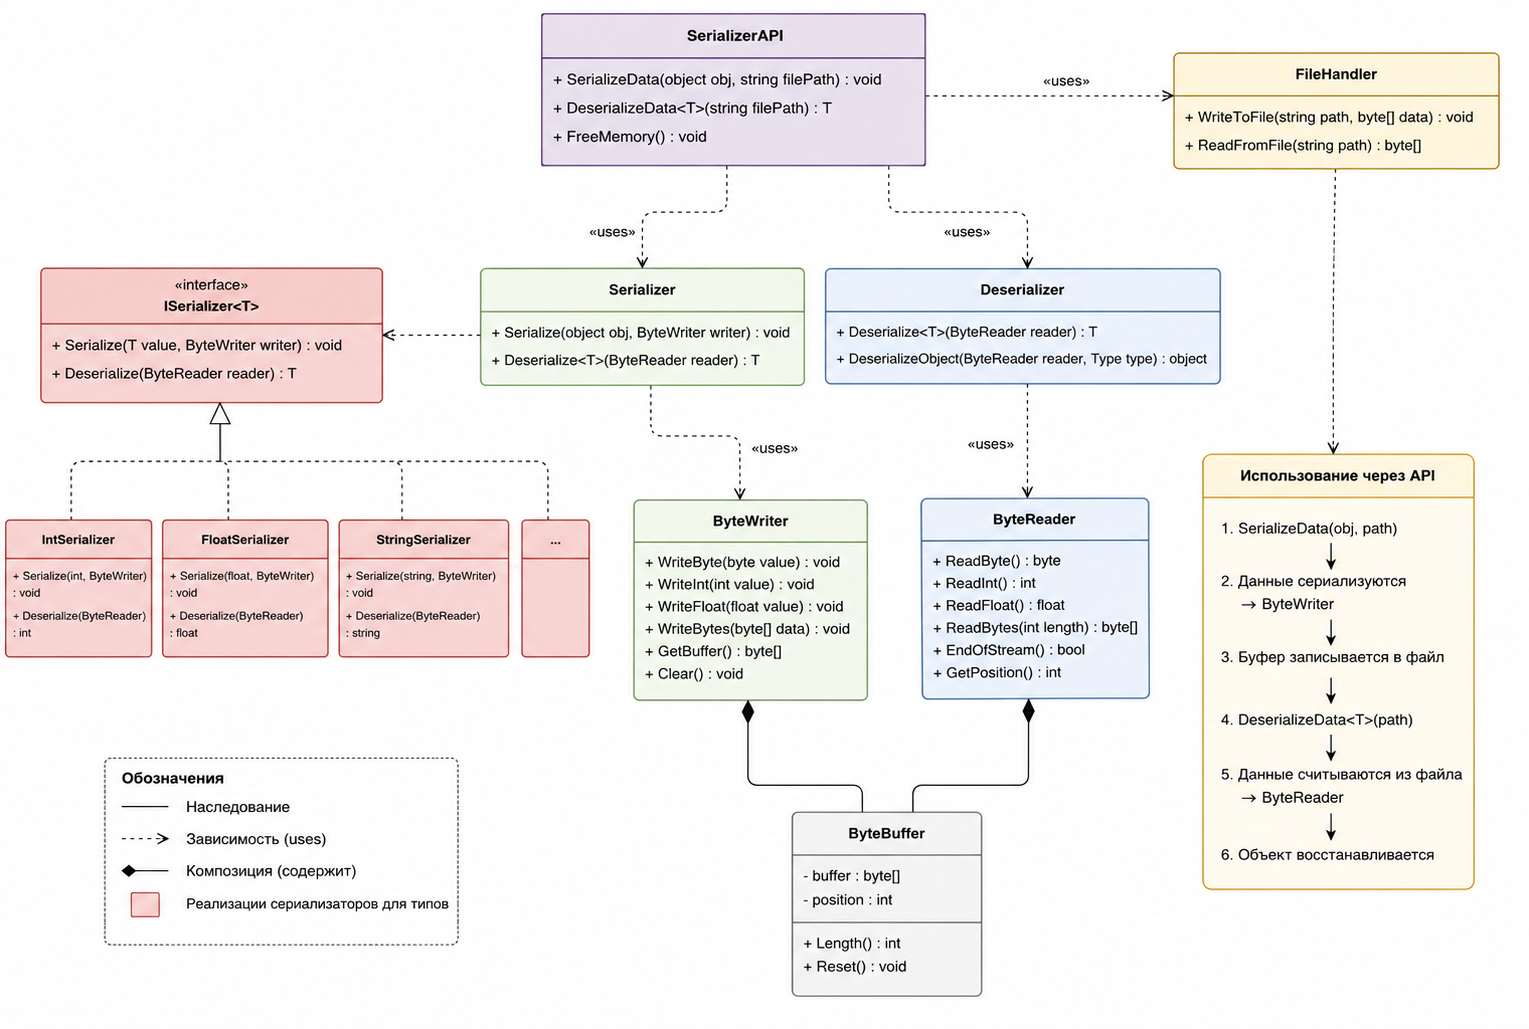
\includegraphics[width=1\linewidth]{UML-диаграмма классов.png}
    \caption{UML-диаграмма классов}
    \label{fig:placeholder}
\end{figure}
\FloatBarrier

\subsubsection{Класс ByteWriter}

Класс \texttt{ByteWriter} реализует функциональность последовательной записи данных в динамический буфер. Основным назначением данного класса является формирование бинарного представления объектов в процессе сериализации.

Внутренняя структура основана на динамическом массиве байтов, в который последовательно записываются значения примитивных типов. Класс предоставляет методы записи отдельных байтов, целых чисел и чисел с плавающей точкой. Все операции выполняются в фиксированном порядке байт (little-endian), что обеспечивает переносимость данных между различными платформами.
\begin{verbatim}
class ByteWriter
{
private:
	std::vector<byte> buffer;
public:
	void clear();
	const std::vector<byte>& getBuffer() const;
	size_t size() const;
	// Write value
	void writeByte(byte value);
	void writeBytes(const byte* data, size_t count);
	void writeInt(int32_t value);
	void writeFloat(float value);
};
\end{verbatim}

\subsubsection{Класс ByteReader}

Класс \texttt{ByteReader} реализует обратную операцию — чтение данных из бинарного буфера. Он хранит ссылку на исходный массив байтов и текущую позицию чтения.

Основной задачей данного класса является последовательное восстановление значений примитивных типов с проверкой корректности границ буфера. При попытке выхода за пределы доступных данных генерируется исключение, что позволяет обнаруживать повреждённые или некорректные файлы на раннем этапе обработки.
\begin{verbatim}
class ByteReader
{
private:
	const std::vector<byte>& data;
	size_t pos;
public:
	ByteReader(const std::vector<byte>& input);
	bool hasMore(size_t count = 1) const;
    // Read value
	byte readByte();
	const byte* readBytes(size_t count);
	int32_t readInt();
	float readFloat();
	size_t getPosition() const;
};
\end{verbatim}

\subsubsection{Система типизации сериализуемых данных}

Для идентификации типов данных в потоке сериализации используется перечисление \texttt{DataType}. Оно позволяет явно маркировать записываемые значения и обеспечивает корректную интерпретацию данных при десериализации.

Каждое сериализуемое значение предваряется идентификатором типа, что делает бинарный формат самодостаточным и позволяет выполнять проверку соответствия ожидаемого и фактического типа данных.

\subsubsection{Сериализаторы примитивных типов}

Для каждого поддерживаемого примитивного типа данных реализован отдельный класс сериализатора. В текущей версии библиотеки представлены следующие реализации:

\begin{itemize}
    \item \texttt{BoolSerializer} — сериализация логических значений;
    \item \texttt{IntSerializer} — сериализация 32-битных целых чисел;
    \item \texttt{FloatSerializer} — сериализация чисел с плавающей точкой.
\end{itemize}

Каждый сериализатор реализует единый интерфейс, включающий операции преобразования данных в бинарный формат и обратного восстановления исходного значения  (статичные методы serialize и deserialize), принимающие объект \texttt{ByteWriter} или \texttt{ByteReader} соответственно. Такой подход позволяет использовать сериализаторы без создания экземпляров классов и обеспечивает единообразный интерфейс работы.

\subsubsection{Сериализация символьных и строковых данных}

Для поддержки текстовой информации реализованы такие классы, как \texttt{CharSerializer} и \texttt{StringSerializer}. Сериализация символа осуществляется как запись одного байта с предварительной маркировкой типа.

Строки сериализуются как последовательность символов с предварительной записью длины строки. Такой подход позволяет однозначно определить границы строки при десериализации и избежать необходимости использования специальных завершающих символов.

Использование явной длины также повышает эффективность чтения и исключает дополнительные операции поиска конца строки.

\subsubsection{Сериализация коллекций}

Для поддержки составных типов данных в библиотеке реализованы обобщённые механизмы сериализации коллекций. В частности, предусмотрены классы \texttt{ArraySerializer}, \texttt{ListSerializer} и \texttt{DictionarySerializer}.

Сериализация последовательных коллекций (массивов и списков) осуществляется путём записи количества элементов, после чего последовательно записываются сами элементы с использованием переданной функции сериализации. Десериализация выполняется в обратном порядке с восстановлением структуры контейнера.

Для ассоциативных контейнеров используется аналогичный подход: сначала записывается количество пар «ключ-значение», затем последовательно сериализуются ключи и значения. Для этого в метод передаются отдельные функции сериализации и десериализации ключей и значений.

Использование шаблонов и функций-указателей позволяет реализовать универсальный механизм работы с коллекциями без жёсткой привязки к конкретным типам данных, что существенно повышает гибкость библиотеки.

\subsubsection{Особенности реализации числовых преобразований}

Сериализация целочисленных и вещественных значений основана на прямом побайтовом представлении данных в памяти. Для целых чисел используется побитовый сдвиг и маскирование, что позволяет последовательно извлекать байты значения.

Для чисел с плавающей точкой используется интерпретация их внутреннего представления согласно стандарту IEEE 754 с последующим преобразованием в целочисленный формат. Это обеспечивает корректное восстановление значений без потери точности при десериализации.

\subsubsection{API взаимодействия с библиотекой}

Взаимодействие с библиотекой осуществляется через набор публичных методов сериализаторов и классов работы с байтовыми потоками. Основной сценарий использования включает создание экземпляра сериализатора, последовательную запись данных в \texttt{ByteWriter} и получение результирующего бинарного буфера.

Обратная операция выполняется через \texttt{ByteReader}, который последовательно восстанавливает значения, контролируя корректность структуры входного потока.

\subsubsection{Расширяемость архитектуры}

Библиотека изначально спроектирована с учётом дальнейшего расширения. Добавление новых типов данных осуществляется путём реализации соответствующих сериализаторов, использующих существующую инфраструктуру работы с байтовым потоком.

Поддержка строк, символов и коллекций демонстрирует возможность масштабирования системы от простых примитивных типов к сложным структурам данных без изменения базовых компонентов.

\subsubsection{Вывод}

Реализованная библиотека представляет собой универсальный инструмент бинарной сериализации, поддерживающий как примитивные, так и составные типы данных. Использование обобщённых механизмов и единообразного API обеспечивает гибкость, расширяемость и возможность применения библиотеки в различных прикладных задачах.

%---------------------------------------------------------------

\subsection{Эксперименты и результаты}

Для оценки эффективности разработанной системы сериализации был проведён ряд экспериментов на различных типах данных, отличающихся структурой, объёмом и характером распределения значений. Это позволяет получить более полное представление о поведении алгоритма в условиях, приближённых к реальным сценариям использования.

В рамках исследования рассмотрены четыре категории данных:
\begin{itemize}
    \item линейные данные;
    \item текстовые данные;
    \item сложные структурированные данные;
    \item смешанные данные.
\end{itemize}

Оценка выполнялась по следующим метрикам: время сериализации, время десериализации и итоговый размер данных.

В рамках эксперимента были включены два стандартных промышленно используемых формата сериализации: XML и DataContractSerializer. Их добавление позволяет получить более репрезентативную картину и провести сравнение не только с упрощёнными текстовыми и бинарными представлениями, но и с типовыми механизмами платформы .NET.

Таким образом, итоговый набор рассматриваемых форматов включает:
\begin{itemize}
    \item бинарный формат (собственная реализация);
    \item JSON (System.Text.Json);
    \item XML (System.Xml.Serialization);
    \item DataContractSerializer (System.Runtime.Serialization);
    \item raw data (прямое представление памяти);
\end{itemize}

Такое разделение позволяет выделить три условные группы: низкоуровневые представления данных (сырые данные и собственная библиотека), универсальные текстовые форматы (JSON и XML), а также платформенно-ориентиро-\newlineванные механизмы сериализации (DataContractSerializer). Подобная классификация используется далее при интерпретации результатов.

При проведении измерений соблюдались следующие условия: единая конфигурация среды выполнения, отключение фоновых процессов, многократное повторение каждого теста с последующим усреднением результатов. Это позволяет снизить влияние случайных отклонений и повысить воспроизводимость эксперимента.
\begin{wrapfigure}{r}{0.5\textwidth}
    \centering
    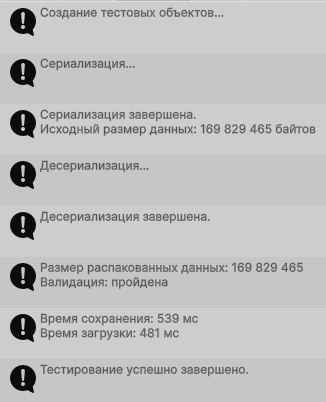
\includegraphics[width=0.5\textwidth]{Logs.png}
    \caption{Логирование сериализации}
    \label{fig:logs}
\end{wrapfigure}
\FloatBarrier

На рисунке \ref{fig:logs} представлен результат тестового запуска разработанной системы сериализации. После сериализации и последующей десериализации выполняется проверка корректности восстановления данных. Совпадение исходных и восстановленных значений подтверждает работоспособность реализованного алгоритма.

\subsubsection{Линейные данные}

В качестве линейного набора данных использовался массив из $10^6$ случайно сгенерированных целых чисел. Данный сценарий моделирует потоковые данные и позволяет оценить накладные расходы сериализации при отсутствии сложных связей между элементами.

Процесс сериализации выполнялся последовательно, без дополнительной обработки структуры. Для каждого формата измерялись временные характеристики и размер результирующего файла.

Результаты эксперимента представлены в таблице \ref{tab:linear_results}.

\begin{table}[h]
\centering
\caption{Результаты для линейных данных}
\label{tab:linear_results}
\begin{tabular}{|c|c|c|c|}
\hline
Формат & Время записи (мс) & Время чтения (мс) & Размер (байт) \\ \hline
Raw data & --- & --- & 6662018  \\ \hline
Binary (custom) & 12 & 12 & 5000005 \\ \hline
JSON & 44 & 51 & 5662028  \\ \hline
XML & 289 & 451 & 21662198  \\ \hline
DataContractSerializer & 215 & 317 & 19662285  \\ \hline
\end{tabular}
\end{table}
\FloatBarrier

\subsubsection{Текстовые данные}

В качестве текстовых данных использовался первый том произведения <<Война и мир>>, представляющий собой последовательность символов значительного объёма. Данный сценарий позволяет оценить эффективность сериализации строк и влияние формата на объём данных.

Результаты приведены в таблице \ref{tab:text_results}.

\begin{table}[h]
\centering
\caption{Результаты для текстовых данных}
\label{tab:text_results}
\begin{tabular}{|c|c|c|c|}
\hline
Формат & Время записи (мс) & Время чтения (мс) & Размер (байт) \\ \hline
Raw data & --- & --- & 1543417 \\ \hline
Binary (custom) & 12 & 12 & 4866915 \\ \hline
JSON & 23 & 21 & 3924624 \\ \hline
XML & 13 & 13 & 3897690 \\ \hline
DataContractSerializer & 41 & 35 & 3959681 \\ \hline
\end{tabular}
\end{table}

\subsubsection{Сложные структурированные данные}

Для моделирования сложных зависимостей была использована структура данных, представляющая граф дорожной сети. Узлы графа соответствуют точкам на карте, а рёбра — соединяющим их участкам. Каждому элементу сопоставлены дополнительные параметры, такие как координаты, тип дороги и вес (длина сегмента).

Данный сценарий отражает особенности сериализации взаимосвязанных объектов, включая необходимость сохранения ссылок и предотвращения дублирования данных.

При проведении эксперимента учитывались:
объём метаданных, влияние структуры графа на размер файла, а также затраты на восстановление связей при десериализации.

Результаты представлены в таблице \ref{tab:graph_results}.

\begin{table}[h]
\centering
\caption{Результаты для графовой структуры}
\label{tab:graph_results}
\begin{tabular}{|c|c|c|c|}
\hline
Формат & Время записи (мс) & Время чтения (мс) & Размер (байт) \\ \hline
Raw data & --- & --- & 7958528  \\ \hline
Binary (custom) & 96 & 93 & 9069010  \\ \hline
JSON & 240 & 246 & 12455876\\ \hline
XML & 690 & 970 & 48678938 \\ \hline
DataContractSerializer & 5890 & 4298 & 45070625 \\ \hline
\end{tabular}
\end{table}

\subsubsection{Смешанный сценарий}

Наиболее приближённым к реальному применению является сценарий, включающий сериализацию сложных объектов, содержащих поля различных типов. В рамках эксперимента использовались реальные классы системы сохранения данных, разработанные для игрового приложения. Объекты включали числовые параметры, строковые данные, вложенные коллекции, а также взаимосвязанные структуры, отражающие состояние различных подсистем.

Для обеспечения достаточного объёма данных и воспроизводимости эксперимента использовался генератор тестовых сущностей, формирующий большое количество объектов с параметрами, соответствующими структуре реальных игровых данных. Такой подход позволил сохранить характер и сложность исходной модели при возможности масштабирования объёма тестируемой информации.

Сырые данные были сохранены в формате JSON в человекочитаемом виде с форматированием, тогда как при измерении производительности сериализация JSON выполнялась без дополнительного форматирования для уменьшения накладных расходов.

Данный сценарий позволяет оценить универсальность разработанного алгоритма и его способность эффективно работать с неоднородными структурами данных, характерными для сложных прикладных систем.

Особое внимание уделялось:
\begin{itemize}
    \item влиянию вложенности на производительность;
    \item накладным расходам на хранение типов данных;
    \item эффективности восстановления объектов;
    \item масштабируемости при увеличении количества сущностей.
\end{itemize}

Результаты приведены в таблице \ref{tab:mixed_results}.

\begin{table}[h]
\centering
\caption{Результаты для смешанных данных}
\label{tab:mixed_results}
\begin{tabular}{|c|c|c|c|}
\hline
Формат & Время записи (мс) & Время чтения (мс) & Размер (байт) \\ \hline
Raw data & --- & --- & 392105984 \\ \hline
Binary (custom) & 582 & 530 & 208284530 \\ \hline
JSON & 5248 & 3980 & 166627620 \\ \hline
XML & 7546 & 7978 & 449783076 \\ \hline
DataContractSerializer & 53533 & 24924 & 346465928 \\ \hline
\end{tabular}
\end{table}

\subsection{Анализ результатов и сравнение с аналогами}

Проведённые эксперименты позволяют оценить эффективность различных подходов к сериализации при работе с данными различной структуры и сложности. Полученные результаты демонстрируют существенные различия между форматами как по скорости обработки, так и по объёму итоговых файлов.

\subsubsection{Общий анализ результатов}

Наиболее стабильные результаты во всех сценариях показала разработанная бинарная библиотека. Во всех тестах собственный бинарный формат демонстрировал минимальное время сериализации и десериализации, а также сохранял сравнительно компактный размер данных. Это объясняется отсутствием промежуточных преобразований, прямой записью байтового представления и минимальным количеством служебной информации.

Текстовые форматы JSON и XML показали значительно более высокие накладные расходы. Основной причиной является необходимость хранения структуры данных в текстовом виде, а также выполнение дополнительных преобразований между строковым и бинарным представлением.

Формат XML продемонстрировал наибольший объём файлов практически во всех тестах. Это связано с высокой избыточностью структуры XML-документов, использованием тегов и необходимостью хранения большого количества служебных элементов.

DataContractSerializer показал промежуточные результаты по размеру файлов, однако оказался наиболее затратным по времени в сложных сценариях. Особенно заметно это проявилось при работе с графовыми структурами и смешанными данными, где время сериализации и десериализации значительно превысило показатели остальных решений.

\subsubsection{Анализ линейных данных}

При сериализации массива из $10^6$ целых чисел различия между форматами оказались особенно заметными. Разработанный бинарный формат обеспечил запись и чтение за 12 мс, что существенно быстрее текстовых решений.

JSON продемонстрировал приемлемые результаты по времени и размеру данных, однако уступил бинарному формату как по скорости, так и по компактности хранения. XML и DataContractSerializer показали значительное увеличение размера файлов — более чем в три раза относительно бинарного представления.

Следует отметить, что raw data в данном эксперименте оказались больше бинарного формата. Это связано с тем, что прямое представление памяти не учитывает оптимизацию структуры хранения и может содержать дополнительные накладные расходы, связанные с особенностями внутреннего представления контейнеров и выравниванием данных.

Полученные результаты подтверждают, что при работе с большими линейными массивами бинарные форматы обладают существенным преимуществом по производительности.

\subsubsection{Анализ текстовых данных}

Результаты эксперимента с текстовыми данными показали иную картину. Несмотря на высокую скорость работы бинарного формата, его итоговый размер оказался больше, чем у JSON и XML.

Причиной этого является специфика реализации строкового сериализатора и особенности кодирования текстовой информации. Текстовые форматы эффективно работают с последовательностями символов и в ряде случаев позволяют избежать дополнительных накладных расходов, возникающих при побайтовом представлении строк.

При этом XML и JSON показали близкие результаты как по времени, так и по размеру файла. DataContractSerializer продемонстрировал более высокие временные затраты, однако размер файла остался сопоставимым с другими текстовыми форматами.

Таким образом, для хранения преимущественно текстовой информации преимущества бинарного представления оказываются менее выраженными.

\subsubsection{Анализ сложных структурированных данных}

Наиболее показательные результаты были получены при сериализации графовой структуры дорожной сети. В данном сценарии существенно возрастает количество взаимосвязей между объектами, а также объём метаданных, необходимых для восстановления структуры.

Разработанная библиотека показала наилучшую масштабируемость: время записи и чтения оставалось сравнительно низким даже при значительном усложнении структуры данных.

JSON продемонстрировал умеренный рост времени и размера файлов, тогда как XML и DataContractSerializer показали крайне высокие накладные расходы. Размер XML-файла превысил бинарное представление более чем в пять раз.

Особенно заметно увеличение времени обработки у DataContractSerializer: сериализация заняла почти 6 секунд, а десериализация — более 4 секунд. Это связано с большим количеством операций отражения типов, проверок структуры объектов и обработки метаданных.

Полученные результаты показывают, что универсальные платформенные механизмы сериализации плохо масштабируются при работе со сложными графовыми структурами.

\subsubsection{Анализ смешанных данных}

Наиболее приближённым к реальным условиям оказался сценарий со смешанными данными, моделирующими состояние игровой системы. В данном тесте использовались объекты с большим количеством полей, строковых данных и вложенных коллекций.

Разработанный бинарный формат вновь продемонстрировал наилучшие временные характеристики: сериализация выполнялась примерно в 9 раз быстрее JSON и более чем в 90 раз быстрее DataContractSerializer.

Однако наиболее интересным результатом стал размер файлов. JSON оказался компактнее бинарного формата и raw data. Это объясняется тем, что в рамках тестирования JSON сохранялся без форматирования, а структура данных содержала большое количество повторяющихся текстовых значений и числовых данных, эффективно представляемых в текстовом виде.

Несмотря на это, бинарная библиотека сохранила значительное преимущество по скорости обработки, что является критически важным для интерактивных приложений и игровых систем.

XML и DataContractSerializer вновь продемонстрировали крайне высокие накладные расходы как по времени, так и по размеру файлов, что ограничивает их применение в системах с частыми сохранениями состояния.

\subsubsection{Сравнение с существующими решениями}

Проведённое исследование показывает, что стандартные механизмы сериализации платформы .NET ориентированы прежде всего на универсальность, совместимость и удобство интеграции. Они позволяют автоматически обрабатывать сложные объектные структуры, однако достигается это ценой снижения производительности.

JSON является компромиссным вариантом между читаемостью и эффективностью. Он обеспечивает сравнительно компактное хранение данных и приемлемую скорость работы, что делает его удобным для обмена информацией и хранения конфигураций.

XML характеризуется высокой избыточностью, однако обладает хорошей формализованностью и расширяемостью. Данный формат остаётся востребованным в системах, где приоритетом является совместимость и строгая структура документов.

Разработанная библиотека ориентирована прежде всего на производительность и минимизацию накладных расходов. За счёт отказа от универсальности и автоматического анализа структуры объектов удалось существенно сократить время обработки данных.

\subsubsection{Применимость результатов к игровым системам}

Полученные результаты показывают, что для игровых приложений и симуляторов наиболее предпочтительными являются специализированные бинарные форматы сериализации.

В системах с большим количеством объектов критически важными являются:
\begin{itemize}
    \item минимальное время сохранения;
    \item высокая скорость загрузки;
    \item снижение объёма данных;
    \item предсказуемое поведение алгоритмов.
\end{itemize}

Разработанная библиотека удовлетворяет данным требованиям значительно лучше универсальных платформенных решений. Это особенно важно для стратегических игр и симуляторов, где состояние мира может включать десятки или сотни тысяч взаимосвязанных объектов.

Текстовые форматы целесообразно использовать преимущественно для отладки, хранения конфигураций и обмена данными между системами.

\subsubsection{Ограничения исследования}

Несмотря на полученные результаты, проведённое исследование имеет ряд ограничений.

Во-первых, эксперименты выполнялись в рамках одной аппаратной и программной конфигурации. Производительность может изменяться в зависимости от архитектуры процессора, объёма оперативной памяти и особенностей среды выполнения.

Во-вторых, в исследовании не рассматривались механизмы предварительного сжатия данных, которые могут существенно изменить соотношение между размером файлов и временем обработки.

В-третьих, разработанная библиотека ориентирована на заранее определённые структуры данных и требует ручной реализации сериализаторов для новых типов, что снижает универсальность решения.

\subsubsection{Перспективы дальнейшего развития}

Дальнейшее развитие библиотеки может быть связано со следующими направлениями:
\begin{itemize}
    \item внедрение поддержки автоматической генерации сериализаторов;
    \item добавление механизмов инкрементального сохранения;
    \item реализация встроенного сжатия данных;
    \item поддержка версионирования форматов;
    \item оптимизация работы со строковыми данными;
    \item поддержка многопоточной сериализации.
\end{itemize}

Дополнительный интерес представляет интеграция библиотеки непосредственно в игровую систему и анализ поведения алгоритма в условиях реальной нагрузки.

\conclusion

В рамках данной курсовой работы были исследованы методы сериализации и хранения данных, а также рассмотрены основные подходы к построению систем сохранения состояния приложений. В ходе исследования были проанализированы требования, предъявляемые к современным механизмам сериализации, включая производительность, компактность хранения, устойчивость к ошибкам, расширяемость и корректность восстановления данных.

В теоретической части работы были рассмотрены особенности различных форматов сериализации, влияние структуры данных на эффективность хранения информации, методы сжатия данных, а также основные метрики оценки производительности систем сериализации. 

Практическая часть работы была посвящена разработке собственной библиотеки бинарной сериализации на языке C++. Реализованная система включает:
\begin{itemize}
    \item механизм последовательной записи и чтения бинарных данных;
    \item поддержку сериализации примитивных типов;
    \item сериализацию строковых данных;
    \item поддержку коллекций и ассоциативных контейнеров;
    \item механизм контроля целостности данных на основе CRC32;
    \item поддержку сжатия данных;
    \item интерфейс взаимодействия с приложением на языке C\# через динамическую библиотеку.
\end{itemize}

Разработанная архитектура позволила обеспечить разделение логики сериализации, повысить расширяемость библиотеки и упростить добавление новых типов данных.

Для оценки эффективности реализованного решения был проведён ряд экспериментов на различных типах данных, включая линейные массивы, текстовые данные, графовые структуры и смешанные объектные модели. Полученные результаты показали, что разработанный бинарный формат обеспечивает существенно более высокую производительность по сравнению с универсальными средствами сериализации платформы .NET.

Наиболее заметное преимущество собственной библиотеки проявилось при работе со сложными структурированными данными, где удалось значительно сократить время сериализации и десериализации, а также уменьшить объём результирующих файлов по сравнению с XML и DataContractSerializer.

В то же время проведённые эксперименты показали, что текстовые форматы, такие как JSON, в отдельных сценариях способны обеспечивать более компактное хранение строковых данных, что связано со спецификой их представления и особенностями тестовых наборов данных. Это подтверждает отсутствие универсального формата сериализации, одинаково эффективного для всех типов информации.

Таким образом, поставленная цель работы была достигнута: были исследованы методы сериализации данных, разработана собственная библиотека бинарной сериализации и проведён сравнительный анализ различных подходов к хранению информации.

Результаты работы показывают, что специализированные бинарные форматы являются наиболее эффективным решением для систем, предъявляющих высокие требования к производительности и скорости сохранения состояния, в частности для игровых приложений, симуляторов и интерактивных систем.


\bibliographystyle{ugost2003}
\bibliography{thesis}


% Окончание основного документа и начало приложений Каждая последующая секция
% документа будет являться приложением

\appendix
\section{Исходные заголовочные файлы библиотеки}
\subsection{SerializerAPI.h}
\begin{verbatim}
#pragma once
#ifdef SERIALIZER_EXPORTS
#define SERIALIZER_API __declspec(dllexport)
#else
#define SERIALIZER_API __declspec(dllimport)
#endif
extern "C"
{
    SERIALIZER_API unsigned char* SerializeData(
        const unsigned char* input,
        int inputSize, int* outputSize
    );
    SERIALIZER_API unsigned char* DeserializeData(
        const unsigned char* input,
        int inputSize, int* outputSize
    );
    SERIALIZER_API void FreeMemory(unsigned char* ptr);
}
\end{verbatim}
\subsection{NumberSerializer.h}
\begin{verbatim}
#pragma once
#include <cstdint>
#include <vector>
#include <string>
namespace Serializer
{
	using byte = uint8_t;
	enum class DataType : uint8_t
	{
		Null=0x00, Bool=0x01, Int=0x02, Float=0x03,
		Char=0x04, String=0x05,
		Array=0x10, List=0x11, Dictionary=0x12,
		Object=0x20
	};
	void SaveToFile(const std::vector<byte>& data,
        const std::string& filename, bool compress = true);
	std::vector<byte> LoadFromFile(const std::string& filename);
	uint32_t crc32(const uint8_t* data, size_t length);
	std::vector<byte> compressData(const std::vector<byte>& input); 
	std::vector<byte> decompressData(const std::vector<byte>& input,
        size_t expectedSize);
	class ByteWriter
	{
	private:
		std::vector<byte> buffer;
	public:
		void clear();
		const std::vector<byte>& getBuffer() const;
		size_t size() const;
		void writeByte(byte value);
		void writeBytes(const byte* data, size_t count);
		void writeInt(int32_t value);
		void writeFloat(float value);
	};
	class ByteReader
	{
	private:
		const std::vector<byte>& data;
		size_t pos;
	public:
		ByteReader(const std::vector<byte>& input);
		bool hasMore(size_t count = 1) const;
		byte readByte();
		const byte* readBytes(size_t count);
		int32_t readInt();
		float readFloat();
		size_t getPosition() const;
	};
	class BoolSerializer
	{
	public:
		static void serialize(ByteWriter& writer, bool value);
		static bool deserialize(ByteReader& reader);
	};
	class IntSerializer
	{
	public:
		static void serialize(ByteWriter& writer, int32_t value);
		static int32_t deserialize(ByteReader& reader);
	};
	class FloatSerializer
	{
	public:
		static void serialize(ByteWriter& writer, float value);
		static float deserialize(ByteReader& reader);
	};
}
\end{verbatim}
\subsection{StringSerializer.h}
\begin{verbatim}
#pragma once
#include "NumberSerializer.h"
#include <string>
namespace Serializer
{
	class CharSerializer
	{
	public:
		static void serialize(ByteWriter& writer, char value);
		static char deserialize(ByteReader& reader);
	};
	class StringSerializer
	{
	public:
		static void serialize(ByteWriter& writer,
            const std::string& value);
		static std::string deserialize(ByteReader& reader);
	};
}
\end{verbatim}
\subsection{CollectionSerializer.h}
\begin{verbatim}
#pragma once
#include <unordered_map>
#include <vector>
#include <list>
#include "NumberSerializer.h"
namespace Serializer
{
    template<typename T>
    using SerializeFunc = void(*)(ByteWriter&, T);
    template<typename T>
    using DeserializeFunc = T(*)(ByteReader&);
    class ArraySerializer
    {
    public:
        template<typename T>
        static void serialize(ByteWriter& writer,
            const std::vector<T>& data,
            SerializeFunc<T> serializer);
        template<typename T>
        static std::vector<T> deserialize(ByteReader& reader,
            DeserializeFunc<T> deserializer);
    };
    class ListSerializer
    {
    public:
        template<typename T>
        static void serialize(ByteWriter& writer,
            const std::list<T>& data,
            SerializeFunc<T> serializer);
        template<typename T>
        static std::list<T> deserialize(ByteReader& reader,
            DeserializeFunc<T> deserializer);
    };
    class DictionarySerializer
    {
    public:
        template<typename K, typename V>
        static void serialize(ByteWriter& writer,
            const std::unordered_map<K, V>& dict,
            SerializeFunc<K> keySerializer,
            SerializeFunc<V> valueSerializer);
        template<typename K, typename V>
        static std::unordered_map<K, V> deserialize(
            ByteReader& reader,
            DeserializeFunc<K> keyDeserializer,
            DeserializeFunc<V> valueDeserializer);
    };
}
#include "CollectionSerializer.cpp"
\end{verbatim}

\end{document}
